\section{Numerical Experiments}
\label{sec:experiments}

For the numerical experiments presented in this chapter, we define a baseline set up. In all experiments, if not differently specified, we keep all the parameters as in the baseline set up. 
The parameter values for these baselines are chosen with trial and error with the following goals:

\begin{itemize}
	\item
	Number of people sufficiently large in order not too have a too large variance over different experiments with same parameters.
	\item
	Reasonable computation time per experiment.
	\item
	Reasonable average number of connections per individual and avoiding cases with a non-strongly connected graph (see Chapter~\ref{sec:mathematical})
\end{itemize}


Table \ref{table:1} summarizes the parameter values for the baseline.
\begin{table}[h!]
\centering
\begin{tabular}{||c | c || c | c ||}
	\hline
	Parameter&Value&Parameter&Value\\
	\hline
	$C$&0.2&Range& $[ 0.1\ n_p,\ 0.1\ n_p]$\\
	nRoot&4&News con. type&$[Local,\ Local]$\\
	$n_p$&100&Similarity&$U(0,1)$\\
	$n_f$&2&Crit. Thinking&$U(0,1)$\\
	$n_r$&2&Influenceability&$U(0,1)$\\
	$x(0)$& $0_{n}$ & &\\
	\hline
\end{tabular}
\newline
\caption{Baseline parameter values. For Range and News connection type, the first component refers to the real news sources and the second component refers to the fake news sources. $U$ denotes the uniform random distribution.}
\label{table:1}
\end{table}


For the experiments where convergence is studied, the following expression was used to determine the steps to convergence $k_{\infty}:$
$$
k_{\infty}=\min k$$
such that
$$ \frac{1}{n_p} \sum_{j=1}^{n_p} \vert x(k+1)_j-x(k)}_j \vert <  \tau
$$
where $\tau$ is the tolerance accepted for steady-state, here
$\tau = 0.0001$. In other words, the system is considered at convergence if the average opinion changes for each node is below $0.01\% $ with respect to the previous step.


\subsection{Instruction Level}
\label{sec:Instr_Level}
The goal of this section is to investigate the effect of the \emph{instruction level} on the population's steady state opinions. The instruction level $L \in [0,1]$ models the capacity of people to identify whether a source is spreading real or fake news. For this experiment, we will assume that the instruction level directly affects the trait \emph{critical thinking}. A function $f$  that maps an instruction level to its corresponding critical thinking probability distribution is defined as:
$$
f: L \to p 
$$
$$
p:= \{g,\ g: [0,1] \to \mathbb{R}_+,\ \int_{0}^{1} g(x) \,dx = 1\}
$$
In order to obtain this mapping, the beta distribution is employed: 
$$
f(L) = \text{Beta}(\alpha(L), \beta(L))\ L \in [0,1]
$$
And therefore:
$$
P(CT_i\in[x,x+dx]) = [f(L)](x) dx \text{ with } x\in [0,1],
$$
where $CT_i$ is the critical thinking parameter for individual i. 
For the Beta distribution, the parameters $\alpha$ and $\beta$ are \textbf{[da completare...]} \acomment{da spiegare: come sono scelti, e il fatto che permettano di creare un buon mapping tra instruction level e pdf.} 
\begin{figure}[!t]
	\centering
	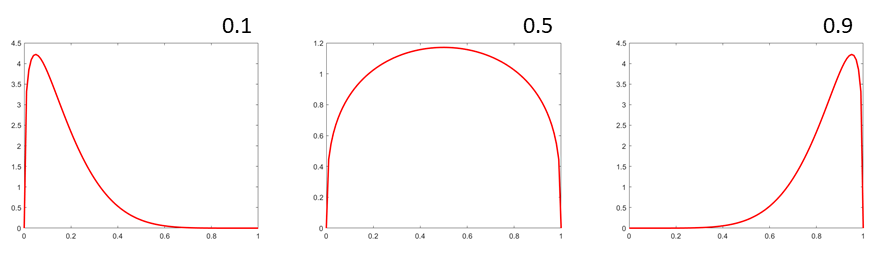
\includegraphics[width=3.5in]{Figures/instruction_level_dist.png}
	\caption{Critical thinking probability distribution for instruction level = \{0.1, 0.5, 0.9\}.}
	\label{pics:critdistribution}
\end{figure}
Figure~\ref{pics:critdistribution} shows the critical thinking probability distribution for three examples of instruction level. A higher instruction level implies, on average, a more critical society with the distribution peak moving to the right (higher critical thinking coefficient). Vice versa, a low instruction level moves the distribution peak to the left (lower critical thinking coefficient). \newline
\begin{figure}[!t]
	\centering
	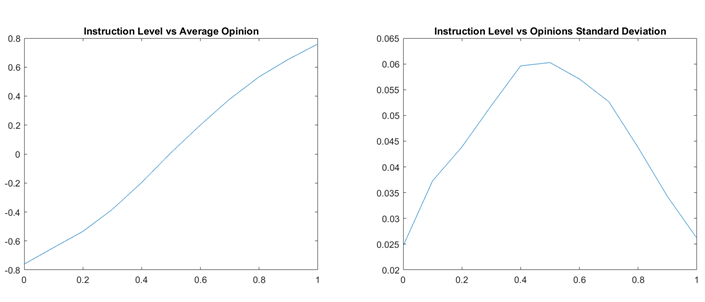
\includegraphics[width=3.5in]{Figures/instruction_results.png}
	\caption{Average opinion and opinions' standard deviation (vertical axis) for instruction level = 0:0.1:1 (horizontal axis).}
	\label{pics:critstatistics}
\end{figure}
In the experiments, the parameter instruction level is varied in its whole range [0,1] and the average opinion and the opinions' standard deviation are computed. The rest of the parameters are left as in Baseline. For each instruction level, 100 cases have been randomly generated and the average metrics have been computed for the steady state opinions.
Figure~\ref{pics:critstatistics} shows the results. As expected, the higher the instruction level, the closer the average opinion is to 1. Vice versa, the lower the instruction level, the closer the average opinion to -1. Furthermore, as the peak gets sharper (either on the right or on the left side) the standard deviation decreases. The opinion therefore converges to values close to 1 (or -1) and the standard deviation decreases as $|L-0.5|$ increases. 
\subsection{Society Diversity}
\label{sec:diversity}
The goal of the numerical experiment presented in this section is investigating the effect of the \textit{diversity factor} $D$ on the transient and steady state behavior of the network opinions. The parameter $D \in \mathbb{R}$ models the diversity of the individuals in the network and will therefore impact the trait \textit{similarity.}
The similarity trait $s_i$ for each individual is drawn from the uniform distribution between $-D$ and $D$:
$$
s_i \backsim U(-D, D),\ D \in \mathbb{R}
$$

The diversity in the society increases as $D$ increases and decreases as $D$ decreases. Each possible similarity value occurs with the same probability but as $D$ increases, the spectrum of possibilities gets larger. \newline
In the experiments, the parameter $D$ is varied in the range [0,50] and the average opinion and the opinions standard deviation are computed. Furthermore the length of the transient phase is recorded. The rest of the parameters are left as in Baseline. For each $D$, 100 networks have been randomly generated and the average metrics have been computed for the steady state opinions, the standard deviations and the time to convergence. 

\begin{figure}[!t]
	\centering
	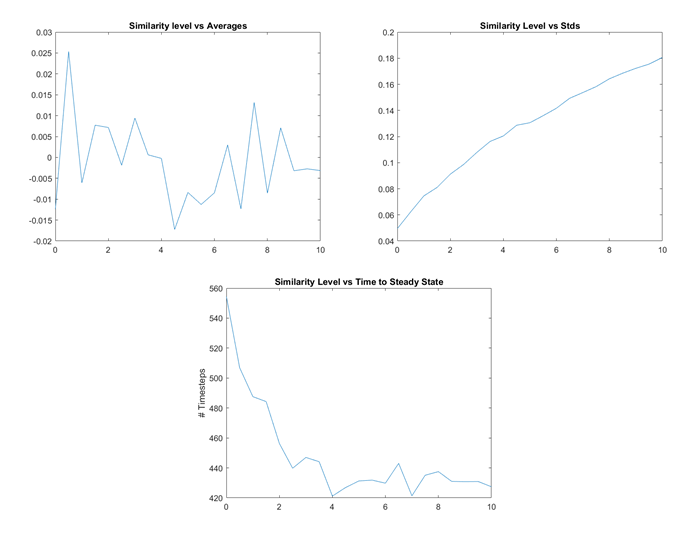
\includegraphics[width=3.5in]{Figures/diversity_results.png}
	\caption{Average Opinion, Opinions Standard Deviation and time to steady state (vertical axis) for $D$ = 0:1:50 (horizontal axis).}
	\label{pics:diversityresults}
\end{figure}
Figure~\ref{pics:diversityresults} illustrates the results. The average opinion does not show any trend as it oscillates with a small amplitude around the value zero, with no bias. This is explainable with the randomness of the network generation. The unbiasedness is expected since no opinion is preferred with this set up. By contrast, the standard deviation increases with $D$. This makes sense, since in a more diverse society, a wider range of opinions is expected. The steady state will therefore show a greater variety of opinions with the resulting larger standard deviation. Finally, the parameter time to steady state shows an initial decrease from $\approx$ 550 to $\approx$ 430 timesteps for $D \in [0,10]$ and then it starts increasing linearly with $D$. The linear increase can be explained by the fact that the weights between different individuals are smaller, and therefore the opinion propagation is slow.

\subsection{Population manipulability}
\label{sec:manipulability}
In this experiment, the goal is to investigate how modifying the \textit{influenceability} trait of the population affects the time to convergence of the opinions in the population. Qualitatively, this would be equivalent to study how well ideas spread in a "stubborn" population versus a highly manipulable population. If one thinks about the real world, the speed of idea spreading is a very important concept. A society with very stubborn individuals may be more stable, and on the other hand change is propelled by people with a flexible view on new ideas.
We define the \textit{manipulability level} $M \in [0,1]$ of the society and study how this affects the time to convergence of the opinion dynamics. A manipulability level of $0$ represents a society difficult to manipulate, while a manipulability level of $1$ represents a society where people are more influenceable. The mapping between $D$ and the population trait \textit{influenceability} is computed through the beta distribution, similarly to the mapping between $L$ and \textit{critical thinking} in Section~\ref{sec:Instr_Level}. For the numerical experiments, the manipulability level is varied in the range $[0,1]$ and the other parameters are left as in Baseline. The experiment is repeated 100 times and the results are averaged. A plot showing that the average time to steady state decreases when the society is more manipulable can be found in Figure~\ref{pics:man_steadystate}. In the range of $M\in [0,1]$, the time to steady state goes from around a maximum of $\approx 580$ timesteps to a minimum of $\approx 480$ timesteps. The result is in line with expectations: the less influenceable individuals are, and the larger weights of the self-loops in the graph will be. For individuals, this corresponds to favoring their own ideas instead of the neighbors' ones and "slowing" thus the information propagation in the network.
This result is in line with the comments made at the beginning of this section, i.e. that ideas spread faster in manipulable societies and slower in less manipulable societies.
\begin{figure}[!t]
	\centering
	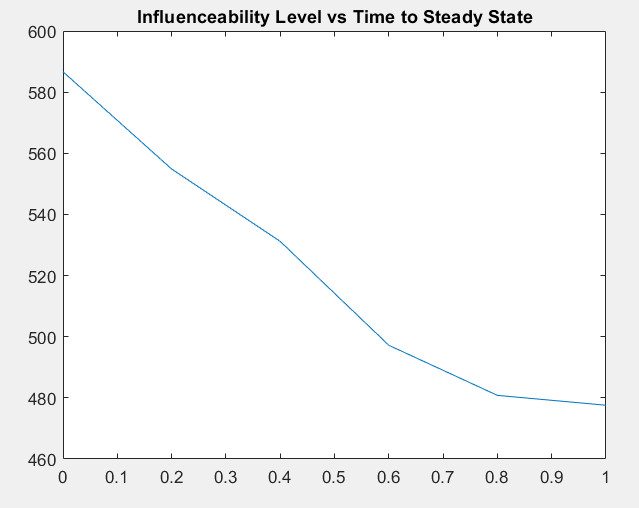
\includegraphics[width=3.5in]{Figures/Exp8_2.png}
	\caption{Average timesteps necessary to reach steady state with varying the manipulability level in the range $[0,1]$.}
\label{pics:man_steadystate}
\end{figure}


\subsection{Polarization}
\label{sec:polarization}
The goal of the numerical experiments presented in this section is investigating the opinion polarization within a population using our model. In particular, we aim to understand how the model parameters influence the polarization. 
Polarization refers either to a distribution of opinions with multiple local maxima or to the process by which such strong divergences of opinions that divide a population come about \cite{Banisch2019}\cite{Bramsona2016}. The model presented in Chapter~\ref{sec:mathematical} has been slightly modified for what concerns the weights between individuals. If $s_i$ denotes the similarity trait of individual $i$, then, at $(S1)$ presented in Section~\ref{sec:conn_ind}, the entry $a_{ij} = a_{ji}$ is 
$$
a_{ij} = \text{max}\{0, \delta_{ij} + 0.2\ r\}
$$
where $r$ is a random number from the normal distribution $\mathcal{N}(0,1)$ and $\delta_{ij} = 1$ if $s_i = s_j$ otherwise $\delta_{ij} = 0$.

The number of real and fake sources is 3. The influenceability and critical thinking traits are set to $0.5$ for all individuals. Similarity is set to $1$ for the first half of individuals in the vector $x$ and to $0$ for the second half. Thus, the probability of creating a link remains the same, but the weight that the link has is around 1 if the nodes belong to the same half and non-negative and close to 0 if they belong to different halves. An example of a single experiment is shown in Figure~\ref{pics:exp20}.\\

\begin{figure}[!t]
\centering
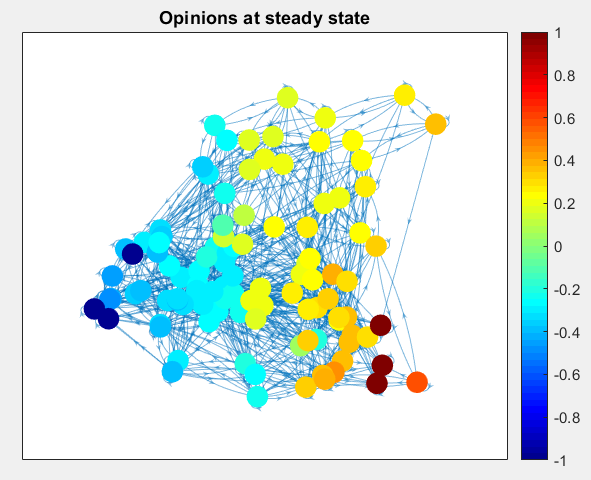
\includegraphics[width=8cm]{Figures/Exp20_graphb.png}
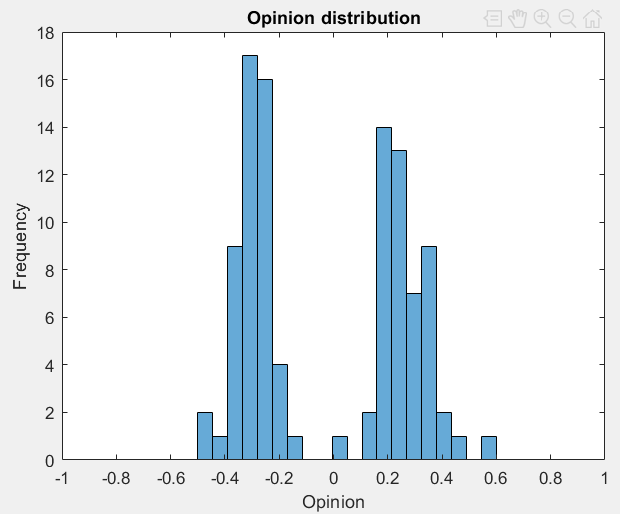
\includegraphics[width=8cm]{Figures/Exp20_hystb.png}
\caption{Simulation with 100 individuals, 3 sources of Fake and 3 of Real News, $C=0.2$, nRoot$=4$ and new connection local. Above: graph at steady state. Below: opinion distribution at steady sate.}
\label{pics:exp20}
\end{figure}

To the best of our knowledge, there is not a unique metric to quantify opinion polarization. We analyzed three metrics: the measure proposed in \cite{Matakos2017} defined as $R_2 = ||x_{\infty}||^2/ N$, the standard deviation of $x_{\infty}$ according to the interpretation of polarization as dispersion exposed in \cite{Bramsona2016} and the mean.\\

In our experiments, we varied three parameters: $C$ in the range $[0.2; 0.6]$, nRoot in the range $[2; 8]$ and the news connection type, which is either local or non-local. For each parameters combination, 100 cases have been randomly generated and the average metrics have been computed for the opinion vector at steady state.\\

The mean is at  $0 \pm 5\times 10^{-3}$ for all cases, which means that there is not a predominant opinion. This is expected, because the parametrization of the personality traits does not favour one opinion. When the news sources have non-local connections, the average is even closer to 0 ($0 \pm 10^{-3}$). Although in this section we are not interested in the average opinion, the fact that the mean is close to 0 supports the choice of using standard deviation and $R_2$ as metrics to evaluate the polarization. A high standard deviation correspond to many entries far from the center on both sides of the opinion spectrum.\\

Because of the mean $\overline{x}$ close to 0 and $N=100$, we have
$$ \sigma^2 = \frac{1}{N-1} \sum_{i=1}^N (x_i-\overline{x})^2 \approx \frac{1}{N} \sum_{i=1}^N x_i^2 = R_2.$$

Thus, the two metrics carry the same information about the polarization and, for the sake of simplicity, we only discuss the standard deviation. Results for 30 parameters combinations are shown in Figure~\ref{pics:pol_std}. Since the opinions are between $-1$ and $1$, the standard deviation is between 0 and 1.\\

We notice that the higher $C$ and nRoot are, the less polarized are the opinions. Moreover, the lower nRoot is, the faster the polarization grows by decreasing $C$. This is in line with our expectations. The higher $C$ is, the more likely contacts are, because $C$ is proportional to the average in and out degree of each node. A high nRoot means that each individual is more likely to have a link with another individual which is far and, in this case, contacts among individuals with different similarity are more likely. Thus, the experiments show that polarization arises in the society when individuals are in contact with few other people or when they are in contact mainly with similar people. The strongest polarization is present when both conditions are met.\\

\begin{figure}
\centering
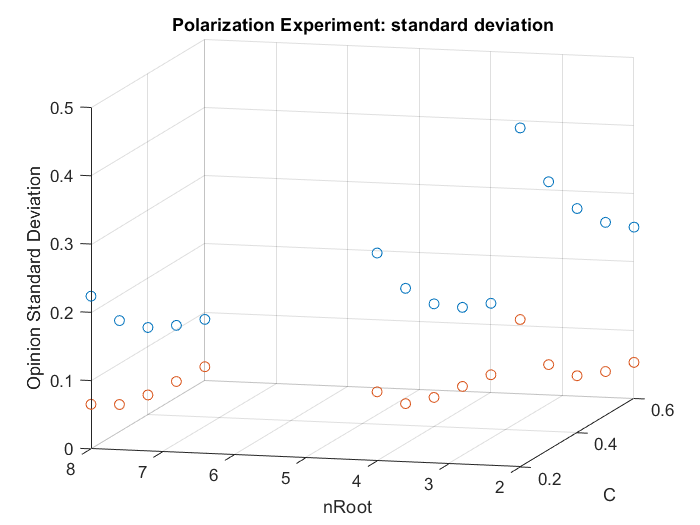
\includegraphics[width=8cm]{Figures/pol_std1.png}
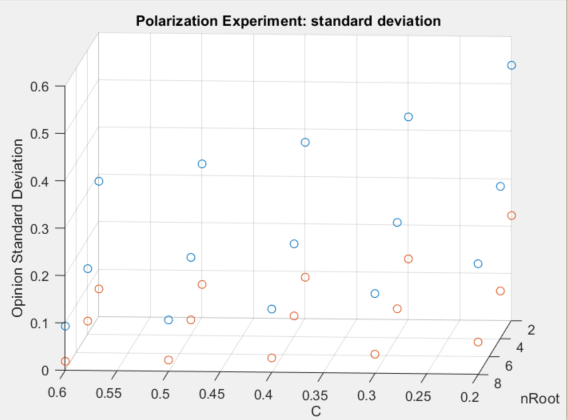
\includegraphics[width=8cm]{Figures/pol_std2.png}
\caption{Standard deviation for different combinations of C, nRoot and news connection. Red: news are spread. Blue: news are local.}
\label{pics:pol_std}
\end{figure}


Another remarkable result is the comparison between the cases where the news connection type is local (blue) and when it is non-local (red). Non-local news connectivity reduces the polarization in the network. This is in line with \cite{Lee2014a}.
For each $C$ and nRoot combination, the standard deviation is at most one third of the value for the corresponding case with local news connectivity. Also with non-local news connectivity, we observe an increase of polarization when $C$ and nRoot decrease, but the growth is less strong. This experiment suggests that a society where each individual has the chance to come in touch with all news sources and not only the ones close to their milieu, is less likely be polarized.

